\chapter{Capa de datos}

El presente capítulo se ocupa de la capa de datos de la arquitectura del Perfil del estudiante. En particular, describe en detalle el proceso de extracción, transformación y carga al que los datos son sometidos. Adicionalmente, provee una perspectiva, a un más alto nivel de abstracción, de cómo los datos fluyen desde su origen hasta su destino final en el Perfil del estudiante, que resulta útil como contexto y preámbulo de los capítulos subsiguientes.

\section{Fuentes de datos}

En aras de que el Perfil del estudiante satisfaga su expectativa como núcleo de información académica y socioeconómica de los estudiantes de la Universidad de los Andes, es necesario que unifique la información que se encuentra dispersa en múltiples sistemas y formatos. En particular, se espera que el Perfil del estudiante sea capaz de reproducir, como mínimo, la información disponible en los sistemas de información académica de la Universidad, como Banner y Advise, así como información en rl sistema de gestión financiera y en el portal de oferta de cursos. La tabla \ref{tab:fuentes_datos} detalla las fuentes de datos cuya información debe ser reproducida por el Perfil del estudiante, incluyendo su nombre formal y una breve descripción de la información que contienen. \cite{advise}

% TODO: Añadir estos parceros, Banner, Advise, Oferta Cursos, al glosario
\begin{table}[h]
	\caption{Fuentes de datos utilizadas por el Perfil del estudiante}
	\centering
	\alternatecolors
	\begin{tabular}{p{0.15\linewidth}p{0.2\linewidth}p{0.65\linewidth}}
		\hline
		\textbf{Nombre}               & \textbf{Nombre Formal}     & \textbf{Descripción}                                                                                                                                                                                                                                                                                                                                                                                                                                       \\
		\hline
		Banner                        & Ellucian Banner            & Sistema de planificación de recursos empresariales (ERP) diseñado para instituciones de educación superior. Es capaz de gestionar procesos académicos y administrativos, incluyendo matrículas, registros académicos, finanzas y recursos humanos. \cite{banner} Almacena el registro académico completo de cada uno de los estudiantes de la Universidad en todos los niveles académicos, así como algunos de los antecedentes académicos del estudiante. \\
		Advise                        & Ellucian CRM Advise        & Sistema de gestión de relaciones con los estudiantes (CRM) que permite a las instituciones identificar y apoyar proactivamente a estudiantes en riesgo, facilitando intervenciones personalizadas para mejorar su éxito académico. \cite{advise}                                                                                                                                                                                                           \\
		Oferta de Cursos              & Portal de Oferta de Cursos & Plataforma web que permite a los estudiantes consultar los cursos disponibles en cada periodo académico, incluyendo información detallada sobre horarios y profesores. \cite{oferta_cursos}                                                                                                                                                                                                                                                                \\
		Sistema de Gestión Financiera &                            & Representación genérica de los sistemas contables y financieros de la universidad, en los que se maneja la información relacionada con becas, créditos educativos y pagos realizados por los estudiantes, al igual que información socioeconómica del estudiante relevante para la asignación de auxilios económicos.                                                                                                                                      \\
		\hline
	\end{tabular}
	\label{tab:fuentes_datos}
\end{table}

% TODO: Añadir Ecosistema de analítica institucional al glosario
Para el acceso a la información contenida en estas fuentes de datos, la Universidad dispone de un Ecosistema de analítica institucional, cuyo propósito es precisamente facilitar el acceso a la información y la generación de conocimiento a partir de los datos. El Ecosistema tiene entre sus objetivos específicos \say{Entregar los datos con estándares de calidad y seguridad para suplir las necesidades de la Universidad}, \say{Hacer el uso de datos para garantizar una toma de decisiones informada} e \say{Impulsar una cultura de uso de datos en la Universidad}. \cite{ecosistema} El uso del Ecosistema evita tener acceder directamente a las fuentes de datos, lo que simplifica el proceso de extracción de datos y terceriza la responsabilidad de la consistencia de los mismos, al menos en su origen, a la Universidad.

Como complemento a lo anterior, teniendo en mente la enorme responsabilidad que recae sobre el Ecosistema respecto a la calidad de los datos, que resulta ser un aspecto crítico para que el Ecosistema pueda cumplir con sus objetivos y en efecto ser útil y confiable a las diversas dependencias de la Universidad, se realizó el esfuerzo de registrar en el apéndice \ref{ap:ecosistema} todos los problemas de calidad de los datos que se han encontrado en el Ecosistema y cómo se han abordado.

%Saltico!

Esa información se encuentra en archivos PARQUET y XLSX almacenados en la nube mediante Microsoft Azure Blob Storage, en diversas cuentas de almacenamiento Azure Storage Account. Para el perfil del estudiante se hace uso de diez de esos archivos, distribuidos en dos cuentas de almacenamiento. Todos los archivos utilizados, junto con su ubicación en cuentas de almacenamiento y directorios, se muestran en la figura \ref{fig:blob_storage}.

\begin{figure}[h]
	\centering
	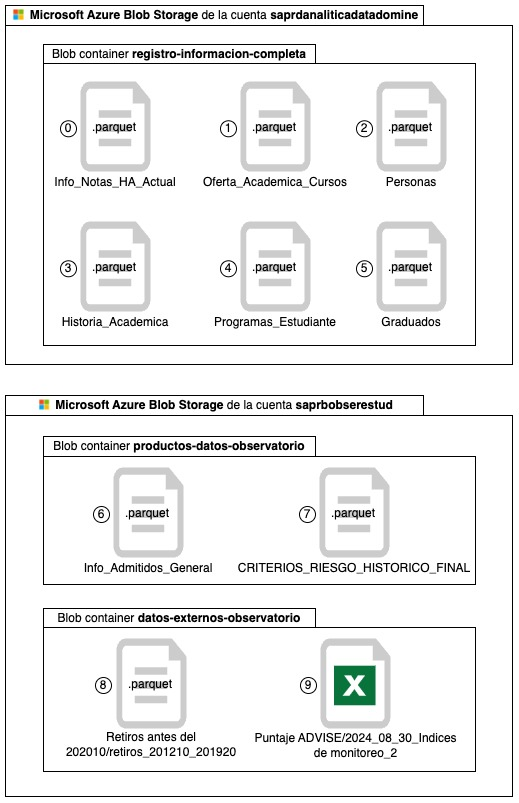
\includegraphics[width=0.7\textwidth]{img/blob_storage.jpg}
	\caption{Archivos fuente y estructura de directorios en Azure Blob Storage}
	\label{fig:blob_storage}
\end{figure}


\section{Proceso de extracción, transformación y carga}

La recuperación y el procesamiento de los datos se realizan mediante un \textit{pipeline} de analítica implementado en cuadernos de Jupyter en Python, en colaboración con los estudiantes Santiago Martínez Novoa y Manuel Felipe Porras Tascón\footnote{Mi más sincero agradecimiento a ambos: a Manuel, en aquel momento estudiante de la Maestría en Ingeniería de la Información, por su valiosa labor al crear y trabajar inicialmente en el cuaderno; y a Santiago, entonces estudiante de Ingeniería de Sistemas y Computación, por tomar la posta, mejorar y mantener este trabajo. Sin ellos, este proyecto no habría sido posible.}.
El pipeline de analítica realiza las tres etapas clásicas de un proceso de \gls{ETL}: extracción, transformación y carga de los datos.


\subsubsection{Extracción de los datos}

El proceso de extracción consiste de tomar información determinada de cada uno de los archivos presentados en la figura \ref{fig:blob_storage}. La tabla \ref{tab:extraccion} detalla el orden en el que se realiza cada extracción, describe la información que se extrae y especifica el archivo fuente del cual se obtiene, empleando la numeración de los archivos definida en la figura \ref{fig:blob_storage}.

\begin{table}[h]
	\centering
	\caption{Extracción de datos}
	\alternatecolors
	\begin{tabular}{cp{2.3cm}p{7cm}c}
		\hline
		\textbf{Orden} & \textbf{Información}                               & \textbf{Descripción}                                                                                                                 & \textbf{Archivos fuente} \\
		\hline
		1              & Histórico académico                                & Información de las notas obtenidas por los estudiantes en cada una de las asignaturas que han cursado.                               & 0                        \\
		2              & Oferta \newline académica                          & Información de las asignaturas que se ofertan en cada uno de los semestres académicos.                                               & 1                        \\
		3              & Estudiantes                                        & Información básica de los estudiantes.                                                                                               & 2, 3, 6                  \\
		4              & Programas académicos                               & Información de los programas académicos en los que se encuentran inscritos los estudiantes.                                          & 4                        \\
		5              & Información \newline adicional \newline de retiros & Información sobre los retiros de los estudiantes para periodos anteriores al 2019-20, que no se encuentra en el Histórico académico. & 8                        \\
		6              & Graduados                                          & Información de los estudiantes que se han graduado.                                                                                  & 5                        \\
		7              & Criterios \newline de riesgo                       & Información de los criterios de riesgo que se utilizan para identificar a los estudiantes en riesgo académico.                       & 7                        \\
		8              & Advise                                             & Información de los estudiantes tomada de la plataforma Advise.                                                                       & 9                        \\
		\hline
	\end{tabular}
	\label{tab:extraccion}
\end{table}

\subsubsection{Transformación de los datos}

\TODO{Sentarme con Santi a describir la transformación de los datos}

\subsubsection{Carga de los datos}

Como última etapa del procesamiento de los datos, una vez han sido transformados, se cargan en dos archivos en el Blob Storage: uno correspondiente a toda la información relacionada con cada estudiante y otro contiene la información de todas las materias cursadas por cada uno de los estudiantes. La figura \ref{fig:blob_storage_post}, que extiende la figura \ref{fig:blob_storage}, muestra la estructura de directorios y archivos en el Blob Storage tras la carga del par de archivos mencionado.

\begin{figure}[h]
	\centering
	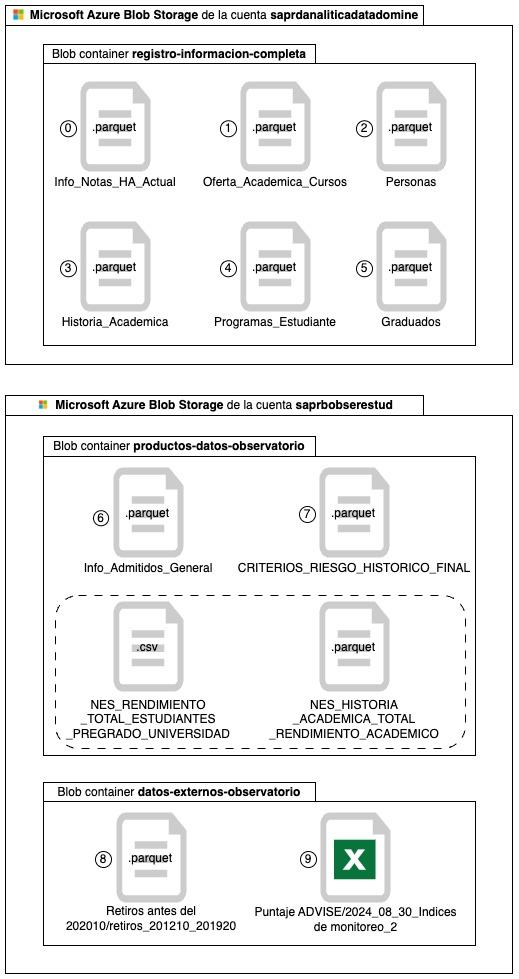
\includegraphics[width=0.7\textwidth]{img/blob_storage_post.jpg}
	\caption{Archivos y estructura de directorios en Azure Blob Storage tras la carga de los datos. Los archivos cargados están encerrados en un rectángulo redondeado con bordes discontinuos.}
	\label{fig:blob_storage_post}
\end{figure}

\section{Flujo de los datos}

La presente sección se ocupa de ofrecer una visión de alto nivel del flujo que los datos atraviesan desde su origen hasta su destino final en el perfil del estudiante. Es sensato presentar este flujo en este punto del documento, pues ya se han detallado las fuentes de datos y el proceso de extracción, transformación y carga de los datos, que es lo que corresponde a la capa de datos de la arquitectura del Perfil del estudiante. Más aún, esta visión general incluye el paso de los datos por el API REST, que es el siguiente componente de la arquitectura del Perfil del estudiante, al igual que el consumo de los datos por parte del frontend. Por ende, esta sección contextualiza al lector y opera como preámbulo a los próximos capítulos.
